\section{\label{quantum-computation}Quantum Computation}

\subsection{Introduction to Qubits}

In contrast to classical computation, where bits form the basis for encoding information, quantum computation makes use of quantum bits (qubits). There are many physical implementations of qubits, however, for the purposes of this thesis, it will suffice to think of them as purely mathematical objects.

Qubits can exist as superpositions of the computational basis: the $\ket 0$ and $\ket 1$ states. These states are orthonormal vectors in a two-dimensional complex Hilbert space $\mathbb{C}^2$. We can depict these states on a Bloch sphere as in figure \ref{zero-state}. Note that the Bloch space does not represent the complex Hilbert space itself.

More generally, we can choose any pair of orthonormal states to form our computational basis. On the bloch sphere, this corresponds to any two vectors pointing in opposite directions. One such computational basis if formed by the $\ket + = \frac{1}{\sqrt{2}} (\ket 0 + \ket 1)$ and $\ket - = \frac{1}{\sqrt{2}} (\ket 0 - \ket 1)$ states.

\begin{figure}[H]
\centering
    \begin{minipage}{.4\textwidth}
      \centering
      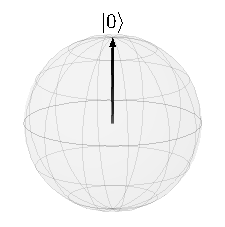
\includegraphics[width=0.5\linewidth]{chapter-1/zero}
      \caption{$\ket 0$ basis state}
      \label{zero-state}
    \end{minipage}%
    \begin{minipage}{.4\textwidth}
      \centering
      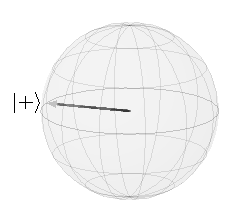
\includegraphics[width=0.5\linewidth]{chapter-1/plus}
      \caption{$\ket +$ basis state}
      \label{plus-state}
    \end{minipage}
\end{figure}
Any qubit $\ket\psi$ can be represented as complex linear combination of the chosen basis, provided that the qubit state vector is normalised.
\begin{equation*}
\begin{gathered}
    \ket \psi = \alpha\ket 0 + \beta\ket 1 \qquad
    |\alpha|^2 + |\beta|^2 = 1 \qquad
    \alpha, \beta \in \mathbb{C}
\end{gathered}
\end{equation*}

\subsection{Multiple Qubit States}
Suppose we have $n$ qubits. By taking the Kronecker product, we can construct $2^n$ computational basis states.
\begin{figure}[H]
\centering
\begin{gather*}
\ket{00 \dots 00} =
\ket{0}_n \otimes \ket{0}_{n-1} \otimes \dots
\otimes \ket{0}_1 \otimes \ket{0}_0 \\[1ex]
%
\dots \\
%
\ket{11 \dots 11} =
\ket{1}_n \otimes \ket{1}_{n-1} \otimes \dots
\otimes \ket{1}_1 \otimes \ket{1}_0
\end{gather*}
\caption{$2^n$ computational basis states.}
\end{figure}

It follows then that any complex linear combination of the computational basis states is also a valid qubit state.
\begin{equation*}
\ket\psi =
\alpha_{00 \dots 00}\ket{00 \dots 00} +
\alpha_{00 \dots 01}\ket{00 \dots 01} +
\dots +
\alpha_{11 \dots 11}\ket{11 \dots 11}
\end{equation*}

Whilst the Bloch sphere representation of a single qubit is incredibly useful, there is no easy generalisation of the Bloch sphere for multiple qubit states \cite{Nielsen2012}.

\subsection{Quantum Gates}
